\documentclass[a4paper, 12pt]{article}%тип документа



%отступы
\usepackage[left=1cm,right=1cm,top=1cm,bottom=2cm,bindingoffset=0cm]{geometry}

%%% Работа с русским языком
\usepackage{graphicx}
\usepackage{cmap}                           % поиск в PDF
\usepackage{mathtext} 			 	       % русские буквы в формулах
\usepackage[T2A]{fontenc}               % кодировка
\usepackage[utf8]{inputenc}              % кодировка исходного текста
\usepackage[english,russian]{babel} 
\usepackage{float}
\usepackage{caption}
\usepackage{multirow} 

\usepackage[export]{adjustbox} % локализация и переносы

\usepackage{subfig}% http://ctan.org/pkg/subfig
\usepackage{booktabs}

\usepackage{wrapfig}


%Матеша
\usepackage{amsmath,amsfonts,amssymb,amsthm,mathtools} % AMS
\usepackage{icomma} % "Умная" запятая

%\mathtoolsset{showonlyrefs=true} % Показывать номера только у тех формул, на которые есть \eqref{} в тексте.

%% Шрифты
\usepackage{euscript}	 % Шрифт Евклид
\usepackage{mathrsfs} % Красивый матшрифт

%% Свои команды
\DeclareMathOperator{\sgn}{\mathop{sgn}}

%% Перенос знаков в формулах (по Львовскому)
\newcommand*{\hm}[1]{#1\nobreak\discretionary{}
	{\hbox{$\mathsurround=0pt #1$}}{}}




\author{Гаврилин Илья Дмитриевич \\
	Б01-101}
\title{\textbf{Работа 2.1.6 \\ 
		Эффект Джоуля-Томсона}}
\begin{document}
	\maketitle
	\section{Аннотация}
	В данной работе было изучено прохождение газа через пористую губку и наблюдение эффекта Джоуля-Томсона. Были получены значения коэффициентов Джоуля-Томсона ($\mu _{д-т.}$) для различных значений температур. Также были оценены коэффициенты a и b в формуле Ван-дер-Ваальса и $T_{инв}$ - температура смены знака эффекта Джоуля-Томсона. Оценены погрешности полученных величин.	
	\section{Теоретические сведения}
	\begin{figure}[H]
		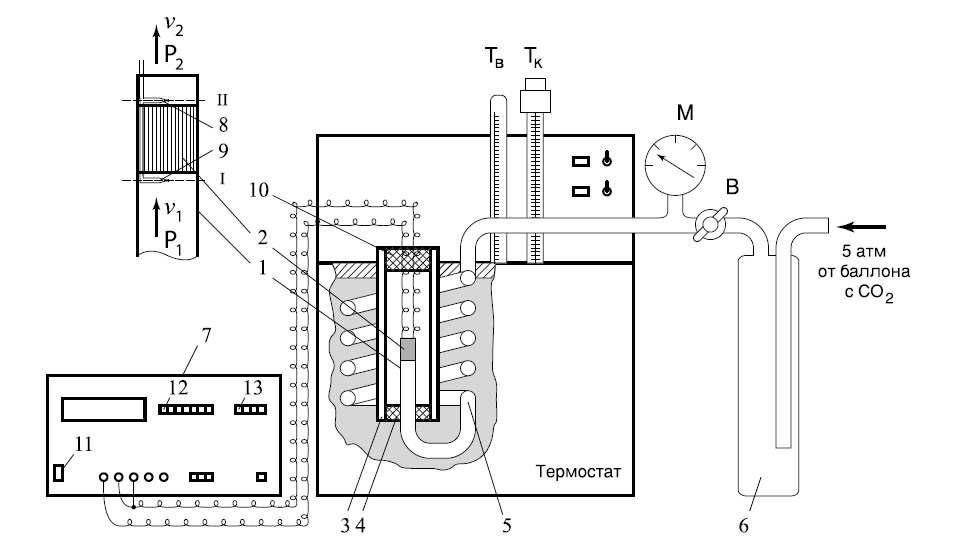
\includegraphics[width = \linewidth]{instrument}
	\end{figure}
	
	
	\section*{Теоретическая часть}
	
	В работе исследуется изменение температуры углекислого газа при медленном его течении по трубке с пористой перегородкой. Трубка 1 хорошо теплоизолирована. Газ из области повышенного давления $P_1$ проходит через множество узких и длинных каналов пористой перегородки 2 в область с атмосферным давлением $P_2$. Перепад давления  $\Delta P = P_1 - P_2$ из-за большого сопротивления
	каналов может быть заметным даже при малой скорости течения газа в трубке. Величина эффекта Джоуля–Томсона определяется по разности температуры газа до и после перегородки.
	
	Рассмотрим стационарный поток газа между произвольными се-
	чениями I и II трубки (до перегородки и после нее). Пусть, для опре-
	деленности, через трубку прошел 1 моль углекислого газа; $\mu$ — его
	молярная масса. Молярные объемы газа, его давления и отнесенные
	к молю внутренние энергии газа в сечениях I и II обозначим соответственно $V_1$ , $P_1$, $U_1$ и $V_2$ , $P_2$ , $U_2$. Для того чтобы ввести в трубку объем $V_1$, над газом нужно совершить работу $A_1$ = $P_1 V_1$. Проходя через сечение II, газ сам совершает работу $A_2$ = $P_2$ $V_2$. Так как через боковые стенки не происходит ни обмена теплом, ни передачи механической
	энергии, то
	\begin{equation}
		A_1-A_2 = \left(U_2+\frac{\mu v_2^2}{2}\right)-\left(U_1+\frac{\mu v_1^2}{2}\right).
	\end{equation}
	В уравнении (1) учтено изменение как внутренней (первые члены в
	скобках), так и кинетической (вторые члены в скобках) энергии газа.
	Подставляя в (1) написанные выражения для $A_1$ и $A_2$ и перегруппировывая члены, найдем
	\begin{equation}
		H_1-H_2 = \left(U + P_1 V_1 \right) - \left(U_2 + P_2 V_2 \right) = \frac{1}{2}\mu\left(v_2^2-v_1^2\right)
	\end{equation}
	
	Сделаем несколько замечаний. Прежде всего отметим, что в процессе Джоуля–Томсона газ испытывает в пористой перегородке существенное трение, приводящее к ее нагреву. Потери энергии на нагрев трубки в начале процесса могут быть очень существенными и сильно искажают ход явления. После того как температура трубки установится и газ станет уносить с собой все выделенное им в пробке тепло, формула (1) становится точной, если, конечно, теплоизоляция трубки достаточно хороша и не происходит утечек тепла наружу через ее стенки.
	
	Второе замечание связано с правой частью (2). Процесс Джоуля–Томсона в чистом виде осуществляется лишь в том случае, если правой частью можно пренебречь, т. е. если макроскопическая скорость газа с обеих сторон трубки достаточно мала. У нас сейчас нет критерия, который позволил бы установить, когда это можно сделать. Поэтому мы отложим на некоторое время обсуждение вопроса о правой части (2), а пока будем считать, что энтальпия газа не меняется.
	
	Рассмотрим выражение:
	\begin{equation}
		\mu_{\text{Д-Т}} = \frac{\Delta T}{\Delta P} \approx \cfrac{\cfrac{2a}{RT}-b}{C_p}
	\end{equation}
	
	Из формулы (3) видно, что эффект Джоуля–Томсона для не очень
	плотного газа зависит от соотношения величин $a$ и $b$, которые оказывают противоположное влияние на знак эффекта. Если силы взаимодействия между молекулами велики, так что превалирует «поправка на давление», то основную роль играет член, содержащий $a$, и
	\[
	\frac{\Delta T}{\Delta P} > 0,
	\]
	то есть газ при расширении охлаждается ($\Delta t < 0$ так как всегда
	$\Delta P < 0$). В обратном случае (малые a):
	\[
	\frac{\Delta T}{\Delta P} < 0,
	\]
	то есть газ нагревается ($\Delta t < 0$ так как по-прежнему
	$\Delta P < 0$).
	
	
	
	Как следует из формул, при температуре $T_i$ коэффициент $\mu_\text{д-т}$ обращается в нуль. Используя связь между коэффици-
	ентами $a$ и $b$ и критической температурой, найдем:
	\begin{equation}
		T_{\text{инв}}=\frac{27}{4}T_{\text{кр}}
	\end{equation}:
	
	При температуре $T_\text{инв}$ эффект Джоуля–Томсона меняет знак: ниже температуры инверсии эффект положителен ($\mu_\text{д-т} > 0$, газ охлаждается), выше $T_\text{инв}$ эффект отрицателен ($\mu_\text{д-т} < 0$, газ нагревается).	
	\section{Ход работы}
	Подготовим установку к работе, прогреем термостат, откроем кран с углекислотой и дождемся установления показаний на вольтметре.\\
	Мы знаем, что чувствительность термопары зависит от температуры, в данной таблицы указаны интервалы в 10 градусов, поэтому позволю себе предположить, что зависимость от температуры можно аппроксимировать линейной функцией, построим такой график и определим функцию для расчета чувствительности при конкретной температуре. 
	\begin{figure}[H]
		\centering
		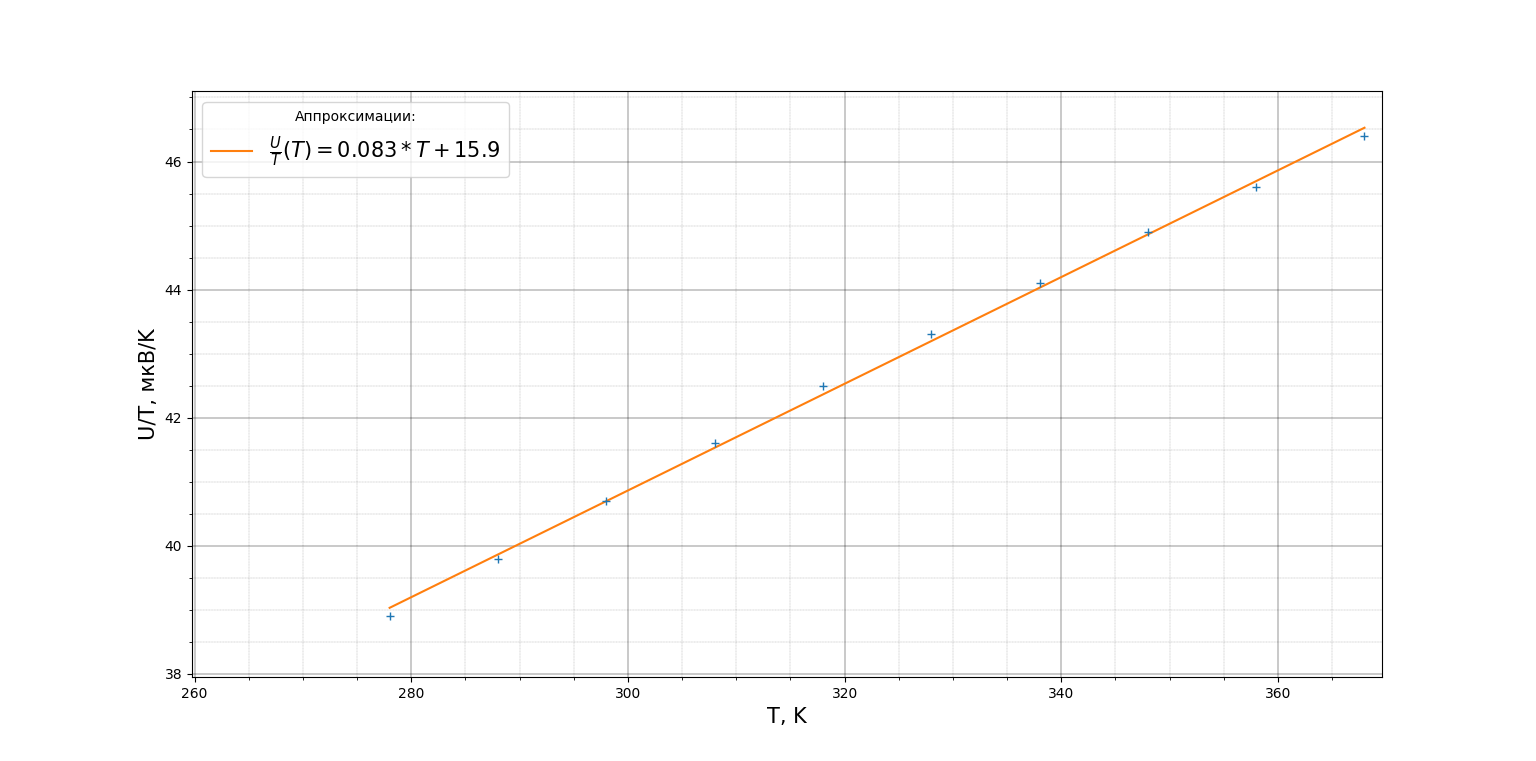
\includegraphics[width=0.9\linewidth]{rt}
		\caption[]{Зависимость чувствительности термопары от температуры}
		\label{fig:rt}
	\end{figure}
	Зависимость действительно в наших пределах температуры может быть аппроксимирована прямой. Поэтому в дальнейшем будем рассматривать чувствительность термопары как функцию температуры.\\
	Тогда проведем замеры для 4 значений температуры(В ходе опытов паразитное эдс было равно $U_0 = 0.002~мВ$):\\
	\begin{table}[H]
		\centering
		\begin{tabular}{|lccccc|}
			\hline
			\multicolumn{6}{|c|}{T   = 293.2 К}                                                                                                                                                 \\ \hline
			\multicolumn{1}{|l|}{$\Delta P, кгс/см^2$}       & \multicolumn{1}{c|}{4}      & \multicolumn{1}{c|}{3.5}    & \multicolumn{1}{c|}{3}      & \multicolumn{1}{c|}{2.5}    & 2                           \\ \hline
			\multicolumn{1}{|l|}{$U-U_0$, мВ}       & \multicolumn{1}{c|}{-0.163} & \multicolumn{1}{c|}{-0.14}  & \multicolumn{1}{c|}{-0.117} & \multicolumn{1}{c|}{-0.092} & -0.072                      \\ \hline
			\multicolumn{1}{|l|}{$\Delta T, K$} & \multicolumn{1}{c|}{4.045}  & \multicolumn{1}{c|}{3.474}  & \multicolumn{1}{c|}{2.903}  & \multicolumn{1}{c|}{2.283}  & 1.787                       \\ \hline
			\multicolumn{6}{|c|}{T = 303.1 К}                                                                                                                                                   \\ \hline
			\multicolumn{1}{|l|}{$\Delta P, кгс/см^2$}       & \multicolumn{1}{c|}{4}      & \multicolumn{1}{c|}{3.5}    & \multicolumn{1}{c|}{3}      & \multicolumn{1}{c|}{2.5}    & 2                           \\ \hline
			\multicolumn{1}{|l|}{$U-U_0$, мВ}       & \multicolumn{1}{c|}{-0.145} & \multicolumn{1}{c|}{-0.124} & \multicolumn{1}{c|}{-0.100} & \multicolumn{1}{c|}{-0.082} & -0.059                      \\ \hline
			\multicolumn{1}{|l|}{$\Delta T, K$} & \multicolumn{1}{c|}{3.526}  & \multicolumn{1}{c|}{3.015}  & \multicolumn{1}{c|}{2.432}  & \multicolumn{1}{c|}{1.994}  & 1.435                       \\ \hline
			\multicolumn{6}{|c|}{T = 313.1 К}                                                                                                                                                   \\ \hline
			\multicolumn{1}{|l|}{$\Delta P, кгс/см^2$}       & \multicolumn{1}{c|}{4}      & \multicolumn{1}{c|}{3.5}    & \multicolumn{1}{c|}{3}      & \multicolumn{1}{c|}{2.5}    & 2                           \\ \hline
			\multicolumn{1}{|l|}{$U-U_0$, мВ}       & \multicolumn{1}{c|}{-0.120} & \multicolumn{1}{c|}{-0.097} & \multicolumn{1}{c|}{-0.070} & \multicolumn{1}{c|}{-0.059} & -0.042                      \\ \hline
			\multicolumn{1}{|l|}{$\Delta T, K$} & \multicolumn{1}{c|}{2.860}  & \multicolumn{1}{c|}{2.312}  & \multicolumn{1}{c|}{1.668}  & \multicolumn{1}{c|}{1.406}  & 1.001                       \\ \hline
			\multicolumn{6}{|c|}{T = 323 К}                                                                                                                                                     \\ \hline
			\multicolumn{1}{|l|}{$\Delta P, кгс/см^2$}       & \multicolumn{1}{l|}{4}      & \multicolumn{1}{l|}{3.5}    & \multicolumn{1}{l|}{3}      & \multicolumn{1}{l|}{2.5}    & \multicolumn{1}{l|}{2}      \\ \hline
			\multicolumn{1}{|l|}{$U-U_0$, мВ}       & \multicolumn{1}{l|}{-0.106} & \multicolumn{1}{l|}{-0.080} & \multicolumn{1}{l|}{-0.061} & \multicolumn{1}{l|}{-0.044} & \multicolumn{1}{l|}{-0.032} \\ \hline
			\multicolumn{1}{|l|}{$\Delta T, K$} & \multicolumn{1}{l|}{2.478}  & \multicolumn{1}{l|}{1.870}  & \multicolumn{1}{l|}{1.426}  & \multicolumn{1}{l|}{1.029}  & \multicolumn{1}{l|}{0.748}  \\ \hline
		\end{tabular}
		\caption{Зависимость разницы температур от избыточного давления}
	\end{table}
	Погрешность определения температуры оценим как: $\sigma (U) = 0.001~мВ; \sigma (\Delta T) = 0.024~K$. Так как, рассчет температуры связан только с погрешностью определения напряжения вольтметром. Определить погрешность чувствительности термопары оценить не представляется возможным.
	Построим график зависимости $\Delta T (\Delta P)$. Перед подстановкой давления проведем его перевод из $кгс/см^2$ в атм.\\
	\begin{figure}[H]
		\centering
		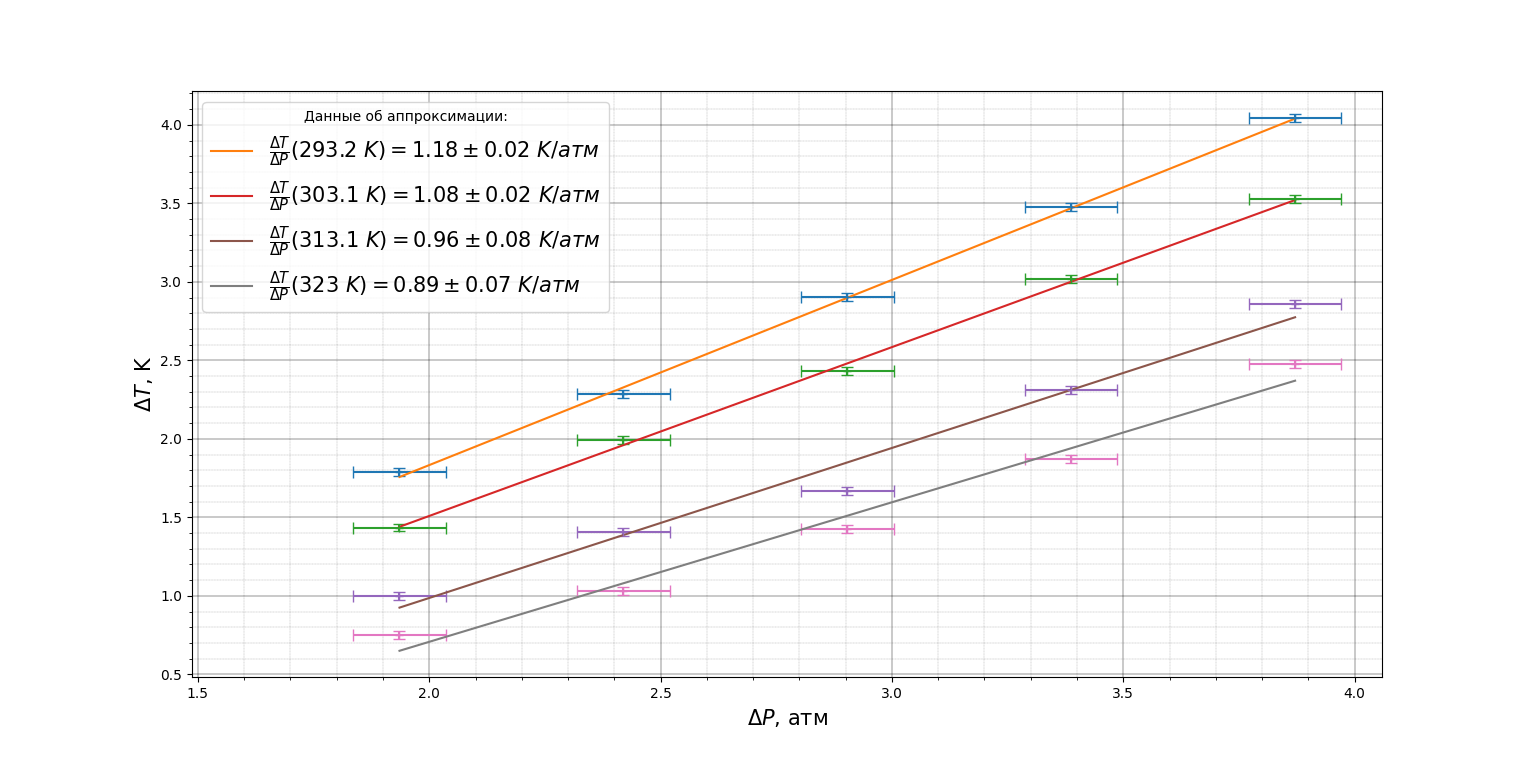
\includegraphics[width=0.95\linewidth]{graph_dj}
		\caption[]{Зависимость разности температур от избыточного давления}
		\label{fig:graphdj}
	\end{figure}
	Итого получили:
	\begin{table}[H]
		\centering
		\begin{tabular}{|c|c|c|c|c|}
			\hline
			T, K  & 293.2     & 303.1     & 313.1     & 323       \\ \hline
			$\mu_{д-т.}$ & $1.18\pm 0.02$ & $1.08\pm 0.02$ & $0.96\pm 0.08$ & $0.89\pm 0.07$ \\ \hline
		\end{tabular}
		\caption{Коэффициент Джоуля-Томсона для углекислого газа при различных температурах}
	\end{table}
	Так как в соответствии формулы (3) коэффициент Джоуля-Томсона обратно пропорционален температуре, для нахождения коэффициентов a, b Ван-дер-Ваальса построим график $\mu_{д-т.}(T) = \frac{K}{T} - B$, с помощью МНК определим K, B.\begin{figure}[H]
		\centering
		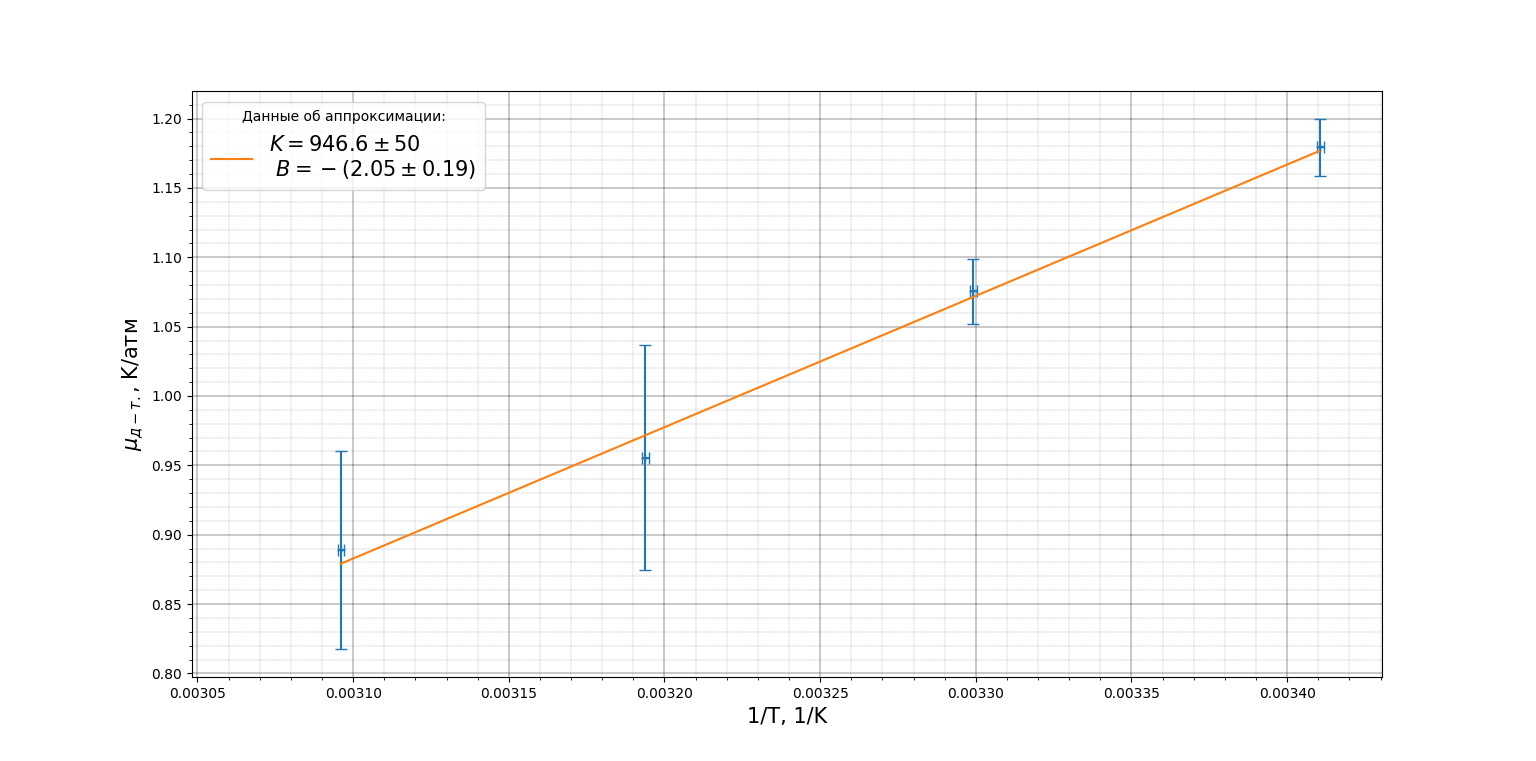
\includegraphics[width=0.9\linewidth]{k_1t}
		\caption{Зависимость коэффициента Джоуля-Томсона от обратной температуры}
		\label{fig:k1t}
	\end{figure}
	Учтем, что коэффициенты K, B определены для давления в атмосферах, при расчете a, b, $T_i$ переведем единицы измерения. Тогда определим коэффициенты a, b и температуру инверсии:\\
	\[
	C_p = 41 \frac{\text{Дж}}{\text{моль} \cdot \text{К}}
	\]
	\[
	a = \frac{KRC_p}{2} = 1.61 \pm 0.08 \frac{\text{Н}\cdot\text{м}^4}{\text{моль}^2} 
	\]
	\[
	b = -BC_p  = (8.4 \pm 0.4)\cdot 10^{-4} \frac{\text{м}^3}{\text{моль}}.
	\]
	\[
	T_i = \frac{2a}{Rb} = 461 \pm 32 K
	\]
	\begin{center}
		Табличное значение:
	\end{center}
	\[
	T_{i_\text{табл}} = 2027 K
	\]
	\section{Выводы}
	1)В ходе работы получили значения a, b и $T_i$ и их погрешности (смотри рассчеты выше).\\
	2)Табличные значения коэф-тов Ван-дер-Ваальса: $a_{табл} = 0.36\frac{\text{Н}\cdot\text{м}^4}{\text{моль}^2};b_{табл}= 0.42\cdot 10^{-4} \frac{\text{м}^3}{\text{моль}}$. Заметим что полученные нами значения не попадают в погрешность. Можно сделать вывод, что несовпадение вызвано методом замеров в котором сложно пренебречь трением молекул, скоростью молекул при выходе, нестационарностью термостата, малым числом замеров.\\ 
	3)Также измеряемый нами диапазон много меньше $T_{i_\text{табл}} = 2027 K$, поэтому замеры коэффициентов a, b могут быть не точными.
\end{document}